\documentclass{beamer}
\usepackage{amsfonts,amsmath,oldgerm}
\usepackage{ragged2e}

\usetheme{sintef}

\newcommand{\testcolor}[1]{\colorbox{#1}{\textcolor{#1}{test}}~\texttt{#1}}

\usefonttheme[onlymath]{serif}

\titlebackground*{assets/background}

\newcommand{\hrefcol}[2]{\textcolor{cyan}{\href{#1}{#2}}}

\title{Aula 00}
\subtitle{2023.1 - SPOIFDS - Informática e Ferramentas para Desenvolvimento }
\course{TÉC. DES. DE SISTEMAS INTEGRADO}
\author{\href{mailto:luizfpq@gmail.com}{Luiz \textbf{Quirino}}}
\IDnumber{luizfpq@gmail.com}



\begin{document}
\maketitle

%\begin{frame}
%
%      Este material é produzido utilizando \LaTeX\, baseado na SINTEF Presentation, disponibilizado sob licenciamento \hrefcol{https://creativecommons.org/licenses/by-nc/4.0/legalcode}{Creative Commons CC BY 4.0}
%
%\vspace{\baselineskip}

%In the following you find a brief introduction on how to use \LaTeX\ and the beamer package to prepare slides, based on the one written by \hrefcol{mailto:federico.zenith@sintef.no}{Federico Zenith} for \hrefcol{https://www.overleaf.com/latex/templates/sintef-presentation/jhbhdffczpnx}{SINTEF Presentation}

% This template is released under \hrefcol{https://creativecommons.org/licenses/by-nc/4.0/legalcode}{Creative Commons CC BY 4.0} license

%\end{frame}

\section{Apresentação}

\begin{frame}{Quem sou eu na fila do pão?}
Formação:
\begin{itemize}
\item Pos-graduação em Gestão de Riscos e CiberSegurança - Focus
\item Sistemas de Informação - UFMS
\item Gestão de Tecnologia da Informação - Unicesumar
\item Técnico em Informática - Centro Paula Souza
\end{itemize}
Atuação:
\begin{itemize}
\item Técnico em Tecnologia da Informação - IFSP
\item Contribuidor OpenSource
\item Desenvolvedor Freelancer
\end{itemize}

\end{frame}

\begin{frame}{Objetivo da disciplina}\justifying
      Descrever e utilizar as principais ferramentas empregadas no desenvolvimento de software como controle de versão, ferramentas de comunicação e redes sociais de desenvolvimento, ferramentas de sistema operacional, editores de texto e ferramentas de escritório.
      
      Configurar e utilizar ambientes integrados de desenvolvimento e suas ferramentas tais como editor e depurador.
      
\end{frame}

\begin{frame}[fragile]{Conteúdo Programático}

\begin{itemize}
      \item Sistemas de controle de versão
      \begin{itemize}
            \item Motivações para controle de versão
            \item Modelos de controle de versão (centralizado e distribuido)
            \item Controle de versão com Git
            \item Estratégias e padronização
      \end{itemize}
      \item Repositórios remotos
      \item Plataformas que usam Git
      \item GitHub Pages
      \item Boas praticas de desenvolvimento de software
      \item Padronização de código
      \item Programação defensiva
\end{itemize}
\end{frame}

\begin{frame}[fragile]{Conteúdo Programático}

      \begin{itemize}
            \item Ferramentas de análise estática
            \item Gerenciamento de dependencias
            \item Terminal e linha de comandos
            \begin{itemize}
                  \item Shell
                  \item Comandos básicos
                  \item Navegação
                  \item Manipulação de arquivos e diretórios
                  \item Configuração de ambiente
            \end{itemize} 
      \end{itemize}
      \end{frame}
      



\section{Planejamento}

\begin{frame}[fragile]{Calendário - Maio}
      \begin{figure}[H]
            \centerline{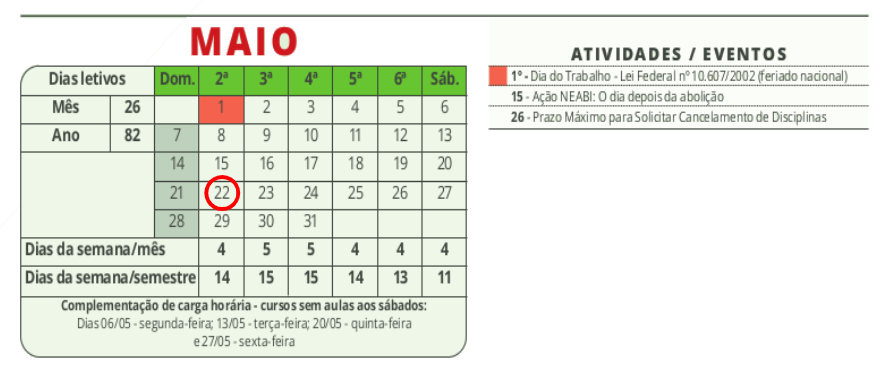
\includegraphics[width=1.1\textwidth]{assets/aula-tads-sopa2-2023-05-22/maio.png}}
            \caption{Calendario academico - maio}
        \end{figure}
\end{frame}


\backmatter
\end{document}
